\documentclass[11pt]{article}

\usepackage{fix-cm}
\usepackage{tikz}
\usetikzlibrary{shapes,backgrounds,calc,patterns}
\usepackage{amsmath,amsthm} 
\usepackage{amssymb}
\usepackage[framemethod=tikz]{mdframed}
% \usepackage{draculatheme}
\usepackage{mathrsfs}
\usepackage{changepage}
\usepackage{multicol}
\usepackage{mathtools}
\usepackage{hyperref}
\usepackage{slashed}
\usepackage{enumerate}
\usepackage{booktabs}
\usepackage{enumitem}
\usepackage{kantlipsum} 
\usepackage{pgfplots}
\pgfplotsset{compat=1.18}
\usetikzlibrary{decorations.markings}

\setlength{\parindent}{0pt}

\newmdenv[
  topline=false,
  bottomline=true,
  rightline=false,
  leftline=true,
  linewidth=1.5pt,
  linecolor=black, % default color, will be overridden in custom commands
  % backgroundcolor=draculabg, % Needed for Dracula theme
  % fontcolor=draculafg, % Needed for Dracula theme
  innertopmargin=0pt,
  innerbottommargin=5pt,
  innerrightmargin=10pt,
  innerleftmargin=10pt,
  leftmargin=0pt,
  rightmargin=0pt,
  skipabove=\topsep,
  skipbelow=\topsep,
]{customframedproof}

\newenvironment{proofpart}[2][black]{
    \begin{mdframed}[
        topline=false,
        bottomline=false,
        rightline=false,
        leftline=true,
        linewidth=1pt,
        linecolor=#1!40, % Custom color
        % innertopmargin=10pt,
        % innerbottommargin=10pt,
        innerleftmargin=10pt,
        innerrightmargin=10pt,
        leftmargin=0pt,
        rightmargin=0pt,
        % skipabove=\topsep,
        % skipbelow=\topsep%
    ]
    \noindent
    \begin{minipage}[t]{0.08\textwidth}%
        \textbf{#2}%
    \end{minipage}%
    \begin{minipage}[t]{0.90\textwidth}%
        \begin{adjustwidth}{0pt}{0pt}%
}{
    \end{adjustwidth}
    \end{minipage}
    \end{mdframed}
}

\newenvironment{solution}
  {\textit{Solution.}}



%%% AESTHETICS %%%
%-%-%-%-%-%-%-%-%-%-%-%-%-%-%-%-%-%-%-%-%-%-%-%-%-%-%-%-%-%-%-%-%-%-%-%-%-%-%


%%% Dimensions and Spacing %%%
\usepackage[left=0.5in,right=0.5in,top=1in,bottom=1in]{geometry}
% \usepackage{setspace}
% \linespread{1}
\usepackage{listings}
% \usepackage{minted}

%%% Define new colors %%%
\usepackage{xcolor}
\definecolor{orangehdx}{rgb}{0.96, 0.51, 0.16}

% Normal colors
\definecolor{xred}{HTML}{BD4242}
\definecolor{xblue}{HTML}{4268BD}
\definecolor{xgreen}{HTML}{52B256}
\definecolor{xpurple}{HTML}{7F52B2}
\definecolor{xorange}{HTML}{FD9337}
\definecolor{xdotted}{HTML}{999999}
\definecolor{xgray}{HTML}{777777}
\definecolor{xcyan}{HTML}{80F5DC}
\definecolor{xpink}{HTML}{F690EA}
\definecolor{xgrayblue}{HTML}{49B095}
\definecolor{xgraycyan}{HTML}{5AA1B9}

% Dark colors
\colorlet{xdarkred}{red!85!black}
\colorlet{xdarkblue}{xblue!85!black}
\colorlet{xdarkgreen}{xgreen!85!black}
\colorlet{xdarkpurple}{xpurple!85!black}
\colorlet{xdarkorange}{xorange!85!black}
\definecolor{xdarkcyan}{HTML}{008B8B}
\colorlet{xdarkgray}{xgray!85!black}

% Very dark colors
\colorlet{xverydarkblue}{xblue!50!black}

% Document-specific colors
\colorlet{normaltextcolor}{black}
\colorlet{figtextcolor}{xblue}

% Enumerated colors
\colorlet{xcol0}{black}
\colorlet{xcol1}{xred}
\colorlet{xcol2}{xblue}
\colorlet{xcol3}{xgreen}
\colorlet{xcol4}{xpurple}
\colorlet{xcol5}{xorange}
\colorlet{xcol6}{xcyan}
\colorlet{xcol7}{xpink!75!black}

% Blue-Purple (should just used colorbrewer...)
\definecolor{xrainbow0}{HTML}{e41a1c}
\definecolor{xrainbow1}{HTML}{a24057}
\definecolor{xrainbow2}{HTML}{606692}
\definecolor{xrainbow3}{HTML}{3a85a8}
\definecolor{xrainbow4}{HTML}{42977e}
\definecolor{xrainbow5}{HTML}{4aaa54}
\definecolor{xrainbow6}{HTML}{629363}
\definecolor{xrainbow7}{HTML}{7e6e85}
\definecolor{xrainbow8}{HTML}{9c509b}
\definecolor{xrainbow9}{HTML}{c4625d}
\definecolor{xrainbow10}{HTML}{eb751f}
\definecolor{xrainbow11}{HTML}{ff9709}

%%% FIGURES %%%
\usepackage{graphicx}  
\graphicspath{ {images/} }  
% \numberwithin{figure}{section}
\usepackage{float}
\usepackage{caption}

%%% Hyperlinks %%%
\usepackage{hyperref}
\definecolor{horange}{HTML}{f58026}
\hypersetup{
	colorlinks=true,
	linkcolor=horange,
	filecolor=horange,      
	urlcolor=horange,
}

\newcommand{\mysqrt}[1]{%
  \mathpalette\foo{#1}%
}
\newcommand{\dmysqrt}[1]{%
  \mathpalette\foodisplay{#1}%
}

\newcommand{\sol}[1]{
    \begin{customframedproof}[linecolor=orangehdx!75,]
        \begin{solution}
        #1
        \end{solution}
    \end{customframedproof}
}
\allowdisplaybreaks

% !TeX spellcheck = off
\newcommand{\foo}[2]{%
  % #1: math style, #2: content
  \sbox0{$#1\sqrt{#2}$}% Measure the size of the standard sqrt in the current style
  \begin{tikzpicture}[baseline=(sqrt.base)]
    \node[inner sep=0, outer sep=0] (sqrt) {$#1\sqrt{#2}$}; % Use the current math style
    \draw([yshift=-0.045em]sqrt.north east) -- ++(0,-0.5ex); % Draw the tick
  \end{tikzpicture}%
}
% !TeX spellcheck = off
\newcommand{\foodisplay}[2]{%
  % #1: math style, #2: content
  \sbox0{$#1\sqrt{#2}$}% Measure the size of the standard sqrt in the current style
  \begin{tikzpicture}[baseline=(sqrt.base)]
    \node[inner sep=0, outer sep=0] (sqrt) {$\displaystyle\sqrt{#2}$}; % Force displaystyle
    \draw[line width=0.4pt] ([yshift=-0.044em]sqrt.north east) -- ++(0,-0.5ex); % Draw the tick
  \end{tikzpicture}%
}

\newcommand{\barNotationT}[1]{\bigg|_{t = #1}}

\newcommand{\cyanit}[1]{\textit{\textcolor{cyan}{#1}}}

\newcommand{\brackett}[1]{\left\langle #1 \right\rangle}

\newcommand{\norm}[1]{\left\lVert \mathbf{#1}\right\rVert}

\newcommand{\mbi}{\mb{i}}
\newcommand{\mbj}{\mb{j}}
\newcommand{\mbk}{\mb{k}}
\newcommand{\mbr}{\mb{r}}
\newcommand{\mbu}{\mb{u}}
\newcommand{\mbv}{\mb{v}}

\newcommand{\vecfuc}[2]{\mb{#1}(#2)}
\newcommand{\dvecfuc}[2]{\mb{#1}'(#2)}
\newcommand{\normdvecfuc}[2]{||\mb{#1}'(#2)||}

\newcommand{\proj}{\text{proj}}

\newcommand{\mb}[1]{\mathbf{#1}}


% \renewcommand{\theenumi}{\arabic{enumi}} 
% \renewcommand{\labelenumi}{\theenumi.}

\title{Multivariable Calculus Exam II Corrections}
\author{Paul Beggs}
\date{April 7, 2025}

%%% Custom Comands %%%
% Natural Numbers 
\newcommand{\N}{\ensuremath{\mathbb{N}}}

% Whole Numbers
\newcommand{\W}{\ensuremath{\mathbb{W}}}

% Integers
\newcommand{\Z}{\ensuremath{\mathbb{Z}}}

% Rational Numbers
\newcommand{\Q}{\ensuremath{\mathbb{Q}}}

% Real Numbers
\newcommand{\R}{\ensuremath{\mathbb{R}}}

% Complex Numbers
\newcommand{\C}{\ensuremath{\mathbb{C}}}

\newcommand{\I}{\ensuremath{\mathbb{I}}}


\begin{document}

\maketitle

\section*{In-Class Portion}

\begin{enumerate}
  \item Consider the function \(\displaystyle f(x,y) = \frac{x^{4} - 4y^{2}}{x^{2} + 2y^{2}}\)
        \begin{enumerate}
          \setcounter{enumii}{1}
          \item (2 points each) We will investigate \(\lim_{(x,y) \rightarrow (0,0)} f(x,y)\).
                \begin{enumerate}
                  \setcounter{enumiii}{1}

                  \item Find the limit, along the path \(y = 0\):

                        \sol{
                          \begin{align*}
                            \lim_{x \to 0} f(x,0) & = \lim_{x \to 0} \frac{x^{4}}{x^{2}} \\
                                                  & = \lim_{x \to 0} x^{2}               \\
                                                  & = \boxed{0}.
                          \end{align*}
                        }

                  \item Find the limit, along the path \(y = x\).

                        \sol{
                          \begin{align*}
                            \lim_{y \to 0} f(y,y) & = \lim_{y \to 0} \frac{y^{4} - 4y^{2}}{y^{2} + 2y^{2}} \\
                                                  & = \lim_{y \to 0} \frac{y^{4} - 4y^{2}}{3y^{2}}         \\
                                                  & = \lim_{y \to 0} \frac{y^{2}(y^{2} - 4)}{3y^{2}}       \\
                                                  & = \lim_{y \to 0} \frac{y^{2} - 4}{3}                   \\
                                                  & = \boxed{-\frac{4}{3}}.
                          \end{align*}
                        }

                  \item What do your answers indicate about this limit?

                        \sol{
                          The limit does not exist, since the limits for each path give different values.
                        }
                \end{enumerate}
        \end{enumerate}
        \newpage
  \item (10 points) Find an equation of the tangent plane to \(g(x,y) = x^{2}e^{x + 2y}\) at point \((2,-1)\).

        \sol{
        First, we need to find the partial derivatives of \(g\):
        \begin{align*}
          g_{x}(x,y) & = \tfrac{\partial}{\partial x} \left[ x^{2}e^{x + 2y} \right]                                                                 \\
                     & = \tfrac{\partial}{\partial x} \left[ x^{2} \right] e^{x + 2y} + x^{2} \tfrac{\partial}{\partial x} \left[ e^{x + 2y} \right] \\
                     & = 2xe^{x + 2y} + x^{2}e^{x + 2y}                                                                                              \\
                     & = e^{x + 2y} \left( 2x + x^{2} \right) \text{, and }                                                                          \\
          g_{y}(x,y) & = \tfrac{\partial}{\partial y} \left[ x^{2}e^{x + 2y} \right]                                                                 \\
                     & = x^{2} \tfrac{\partial}{\partial y} \left[ e^{x + 2y} \right]                                                                \\
                     & = 2x^{2}e^{x + 2y}.
        \end{align*}
        Now that we have our partials, we can evaluate them at the point \((2,-1)\):
        \begin{align*}
          g_{x}(2,-1) & = e^{2 - 2} \left( 2(2) + (2)^{2} \right) \\
                      & = e^{0} \left( 4 + 4 \right)              \\
                      & = 8, \text{ and}                          \\
          g_{y}(2,-1) & = 2(2^{2})e^{2 - 2}                       \\
                      & = 8e^{0}                                  \\
                      & = 8.
        \end{align*}
        We also need to find \(z_{0}\), which is given by solving \(g(2,-1)\):
        \[
          z_{0} = g(2,-1) = 2^{2}e^{2 - 2} = 4e^{0} = 4.
        \]
        Finally, we can write the equation of the tangent plane:
        \[
          \boxed{z = 4 + 8(x - 2) + 8(y + 1).}
        \]
        }
        \newpage
  \item (10 points) Find the directional derivative of \(h(x) = \mysqrt{x + y} - x^{2} + \frac{1}{\pi}\sin(\pi y)\), at the point \((3,1)\) in the direction \(\langle 5, -2 \rangle\).

        \sol{
          Similar to the previous problem, we need to find the partial derivatives of \(h\):
          \begin{align*}
            h_{x}(x,y) & = \frac{\partial}{\partial x} \left[ \mysqrt{x + y} - x^{2} + \frac{1}{\pi}\sin(\pi y) \right] \\
                       & = \frac{1}{2\mysqrt{x + y}} - 2x \text{, and}                                                  \\
            h_{y}(x,y) & = \frac{\partial}{\partial y} \left[ \mysqrt{x + y} - x^{2} + \frac{1}{\pi}\sin(\pi y) \right] \\
                       & = \frac{1}{2\mysqrt{x + y}} + \cos(\pi y).
          \end{align*}
          Then, we evaluate them at the point \((3,1)\):
          \begin{align*}
            h_{x}(3,1) & = \frac{1}{2\mysqrt{3 + 1}} - 2(3)      \\
                       & = \frac{1}{4} - 6                       \\
                       & = -\frac{23}{4}, \text{ and}            \\
            h_{y}(3,1) & = \frac{1}{2\mysqrt{3 + 1}} + \cos(\pi) \\
                       & = \frac{1}{4} - 1                       \\
                       & = -\frac{3}{4}.
          \end{align*}
          Before we can build the directional derivative, we need to find the magnitude of \(\langle 5, -2 \rangle\):
          \[
            \|\mb{v} \| = \| \langle 5, -2 \rangle \| = \mysqrt{5^{2} + (-2)^{2}} = \mysqrt{25 + 4} = \mysqrt{29}.
          \]
          Now we can build the directional derivative:
          \begin{align*}
            D_{\mathbf{v}} & = \frac{(h_{x}(3,1) + h_{y}(3,1)) \cdot \mb{v}}{\mysqrt{29}} \\
                           & = \frac{-\frac{23}{4}(5) - \frac{3}{4}(-2)}{\mysqrt{29}}     \\
                           & = \frac{-\frac{115}{4} + \frac{6}{4}}{\mysqrt{29}}           \\
                           & = \frac{-\frac{109}{4}}{\mysqrt{29}}                         \\
                           & = \boxed{-\frac{109}{4\mysqrt{29}}}.
          \end{align*}
        }
        \newpage

  \item (12 points) For the function \(k(x,y) = x^{3} - 3x + 3xy^{2}\), find each critical point, and identify each as a local minimum, local maximum, or saddle point. [I guarantee there will be no ``inconclusive.'']

        \sol{
          We start by finding the partial derivatives of \(k\):
          \begin{align*}
            k_{x}(x,y) & = 3x^{2} - 3 + 3y^{2}, \\
            k_{y}(x,y) & = 6xy.
          \end{align*}
          From the second equation, we see that either \(y = 0\) or \(x = 0\). If \(y = 0\), then we have:
          \begin{align*}
            k_{x}(x,0) & = 3x^{2} - 3 \\
                       & = 0          \\
            x^{2}      & = 1          \\
            x          & = \pm 1.
          \end{align*}
          If \(x = 0\), then we have:
          \begin{align*}
            k_{x}(0,y) & = -3 + 3y^{2} \\
                       & = 0           \\
            y^{2}      & = 1           \\
            y          & = \pm 1.
          \end{align*}
          So, we have the following critical points:
          \begin{align*}
            (1,0), (-1,0), (0,1), (0,-1).
          \end{align*}
          Now we need to find the second partial derivatives:
          \begin{align*}
            k_{xx}(x,y) & = 6x, \\
            k_{yy}(x,y) & = 6x, \\
            k_{xy}(x,y) & = 6y.
          \end{align*}
          We will use the following equation for \(D\) in order to classify our critical points:
          \[
            D = k_{xx}(x_{0},y_{0})k_{yy}(x_{0},y_{0}) - \bigl(k_{xy}(x_{0},y_{0})\bigr)^{2}.
          \]
          Thus, we get the following table:
          \begin{center}
            \begin{tabular}{ccc}
              \toprule
              \textbf{Critical Point} & \textbf{D}                         & \textbf{Conclusion}                                                \\ \midrule
              \((1,0)\)               & \(6(1)(6(1)) - (6(0))^{2} = 36\)   & \((D > 0) \, \wedge \, (f_{xx} > 0) \, \Rightarrow\) Local minimum \\ \midrule
              \((-1,0)\)              & \(6(-1)(6(-1)) - (6(0))^{2} = 36\) & \((D > 0) \, \wedge \, (f_{xx} < 0) \, \Rightarrow\) Local minimum \\ \midrule
              \((0,1)\)               & \(6(0)(6(0)) - (6(1))^{2} = -36\)  & \((D < 0) \Rightarrow\) Saddle point                               \\ \midrule
              \((0,-1)\)              & \(6(0)(6(0)) - (6(-1))^{2} = -36\) & \((D < 0) \Rightarrow\) Saddle point                               \\ \bottomrule
            \end{tabular}
          \end{center}
        }
        \newpage

  \item (10 points) Find the value of \(\iint_{D} 12xy^{2} \, dA\) where \(D\) is the region in the first quadrant between \(y = x\) and \(y = x^{3}\).

        \sol{
          Our region \(D\) is bounded by the first quadrant and the curves \(y = x\) and \(y = x^{3}\):

          \begin{center}
            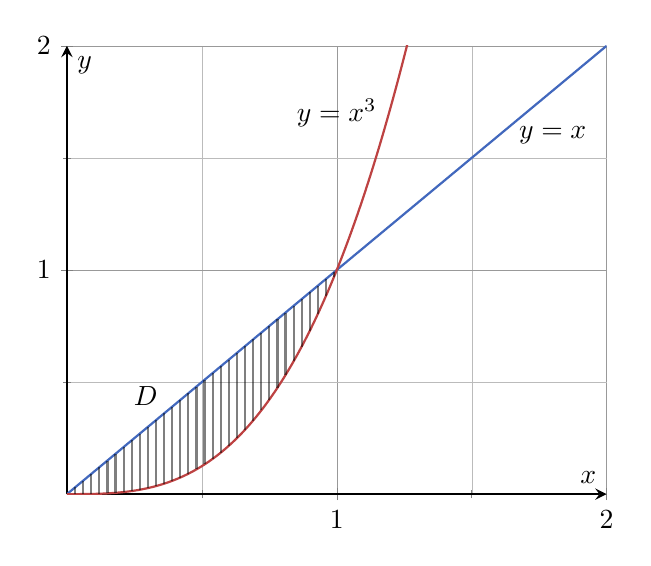
\begin{tikzpicture}
              \begin{axis}
                [axis lines = middle,
                  xlabel = \(x\),
                  ylabel = \(y\),
                  xtick={0,1,2},
                  ytick={0,1,2},
                  xmin=0, xmax=2,
                  ymin=0, ymax=2,
                  domain=0:2,
                  samples=100,
                  thick,
                  grid = both,
                  grid style={line width=.1pt, draw=xgray!50},
                  major grid style={line width=.2pt,draw=xgray!75},
                  minor tick num=1]
                \addplot[domain=0:2,smooth,samples=100,color=xblue,thick] {x};
                \addplot[domain=0:2,smooth,samples=100,color=xred,thick] {x^3};

                \foreach \x in {0,0.03,...,1} {
                  \addplot[black,opacity=0.5] coordinates {(\x,\x^3) (\x,\x)};
                }
                \node at (axis cs:1,1.7) {$y = x^{3}$};
                \node at (axis cs:1.8,1.6) {$y = x$};
              \end{axis}
              \node[above] at (1,1) {$D$};

            \end{tikzpicture}
          \end{center}

          Thus, this gives us the region \(D = \{(x,y) \, | \, 0 \leq x \leq 1, x^{3} \leq y \leq x\}\). \\

          Allowing us to write the double integral as:
          \begin{align*}
            \iint_{D} 12xy^{2} \, dA & = \int_{0}^{1} \int_{x^{3}}^{x} 12xy^{2} \, dy \, dx                            \\
                                     & = \int_{0}^{1} 4x \left[ y^{3} \right]_{x^{3}}^{x} \, dx     \\
                                     & = 4\int_{0}^{1} x \left[ x^{3} - (x^{3})^{3} \right] \, dx \\
                                     & = 4\int_{0}^{1} x^{4}(1 - x^{6}) \, dx                                          \\
                                     & = 4\left[ \frac{x^{5}}{5} - \frac{x^{7}}{7} \right]_{0}^{1}                     \\
                                     & = 4\left( \frac{1}{5} - \frac{1}{7} \right)                                     \\
                                     & = 4\left( \frac{2}{35} \right)                                                  \\
                                     & = \boxed{\frac{8}{35}}.
          \end{align*}
        }
\newpage
  \item (10 points) The solid \(E\) is the region in the cylinder \(x^{2} + y^{2} = 1\) which lives below the plane \(z = 4\) and above \(z = 1 - x^{2} - y^{2}\). [See picture]. Determine \(\iiint_{E} (x^{2} + y^{2}) \, dV\).

        \sol{
          First, we can change our integral to cylindrical coordinates:
          \begin{align*}
            x & = r\cos(\theta), \\
            y & = r\sin(\theta), \\
            z & = z, \\
            dV & = r \, dr \, d\theta \, dz.
          \end{align*}
          Thus, we can rewrite and solve our integral:
          \begin{align*}
            \iiint_{E} (x^{2} + y^{2}) \, dV & = \int_{0}^{2\pi} \int_{0}^{1} \int_{1 - r^{2}}^{4} (r^{2}) \cdot (r) \, dz \, dr \, d\theta \\
                                             & = \int_{0}^{2\pi} \int_{0}^{1} r^{3} \left[ z \right]_{1 - r^{2}}^{4} \, dr \, d\theta \\
                                             & = \int_{0}^{2\pi} \int_{0}^{1} r^{3}\bigl(4 - (1 - r^{2})\bigr) \, dr \, d\theta \\
                                             & = 2\pi\int_{0}^{1} r^{3}(3 + r^{2}) \, dr \\
                                             & = 2\pi\left[ \frac{3r^{4}}{4} + \frac{r^{6}}{6} \right]_{0}^{1} \\
                                             & = 2\pi\left( \frac{3}{4} + \frac{1}{6} \right) \\
                                             & = 2\pi\left( \frac{9}{12} + \frac{2}{12} \right) \\
                                             & = 2\pi\left( \frac{11}{12} \right) \\
                                             & = \boxed{\frac{11\pi}{6}}.
          \end{align*}
          (Note the change in order of integration from \(dr \, d\theta \, dz\) to \(d\theta \, dr \, dz\). This is because the limits of integration for \(z\) are dependent on \(r\), and the limits of integration for \(r\) are dependent on \(\theta\).)
        }

\end{enumerate}


\end{document}